% Copyright 2004 by Till Tantau <tantau@users.sourceforge.net>.
%
% In principle, this file can be redistributed and/or modified under
% the terms of the GNU Public License, version 2.
%
% However, this file is supposed to be a template to be modified
% for your own needs. For this reason, if you use this file as a
% template and not specifically distribute it as part of a another
% package/program, I grant the extra permission to freely copy and
% modify this file as you see fit and even to delete this copyright
% notice. 

\documentclass[aspectratio=169]{beamer}
%\documentclass{beamer}

\setbeamersize{text margin left=10mm, text margin right=10mm}

\defbeamertemplate{headline}{my header}{%
\vskip1pt%
\makebox[0pt][l]{\,\insertshortauthor}%
\hspace*{\fill}\insertshorttitle/\insertshortsubtitle\hspace*{\fill}%
\llap{\insertpagenumber/\insertpresentationendpage\,}
}
\setbeamertemplate{headline}[my header]

\usepackage{arydshln}
\usepackage{graphicx}
\usepackage{soul}
\usepackage{tkz-euclide}
\usetikzlibrary{calc}
\usepackage[]{algorithm2e}
\usepackage{changepage}
\usepackage{amssymb}
\usepackage{xcolor}
\usepackage{mathtools}
\usepackage{tcolorbox}
\usepackage{tikz}
\usetikzlibrary{arrows}
\usepackage{textcomp}
\usetikzlibrary{shapes}
\usepackage{tikz-3dplot}
\usepackage{tkz-euclide}
\usepackage{circuitikz}
\usepackage{pgfplots}
\pgfplotsset{width=7cm,compat=1.8}
\usetikzlibrary{positioning}
\usepackage[tikz]{bclogo}
\presetkeys{bclogo}{
ombre=false,
epBord=0,
couleur = black!10!white,
couleurBord = red,
arrondi = 0.1,
logo=,
}{}
% \usepackage[math]{cellspace}
% \cellspacetoplimit 4pt
% \cellspacebottomlimit 4pt
%\usetikzlibrary{arrows.meta}
% sqare of half axes
\newcommand{\asa}{3}
\newcommand{\bsa}{1}
\newcommand{\csa}{0.25}
% view angle
\tdplotsetmaincoords{70}{135}

%\setbeamertemplate{itemize items}{-}

%\usepackage{helvet}
\usefonttheme{professionalfonts} % using non standard fonts for beamer
%\usefonttheme{serif} % default family is serif
%\usepackage{fontspec}
%\setmainfont{Liberation Serif}

% There are many different themes available for Beamer. A comprehensive
% list with examples is given here:
% http://deic.uab.es/~iblanes/beamer_gallery/index_by_theme.html
% You can uncomment the themes below if you would like to use a different
% one:
%\usetheme{AnnArbor}
%\usetheme{Antibes}
%\usetheme{Bergen}
%\usetheme{Berkeley}
%\usetheme{Berlin}
%\usetheme{Boadilla}
%\usetheme{boxes}
%\usetheme{CambridgeUS}
%\usetheme{Copenhagen}
%\usetheme{Darmstadt}
%\usetheme{default}
%\usetheme{Frankfurt}
%\usetheme{Goettingen}
%\usetheme{Hannover}
%\usetheme{Ilmenau}
%\usetheme{JuanLesPins}
%\usetheme{Luebeck}
%\usetheme{Madrid}
%\usetheme{Malmoe}
%\usetheme{Marburg}
%\usetheme{Montpellier}
%\usetheme{PaloAlto}
%\usetheme{Pittsburgh}
%\usetheme{Rochester}
%\usetheme{Singapore}
%\usetheme{Szeged}
%\usetheme{Warsaw}

% Definition of blocks:
\tikzset{%
  block/.style    = {draw, thick, rectangle, minimum height = 3em,
    minimum width = 3em},
  sum/.style      = {draw, circle, node distance = 2cm}, % Adder
  input/.style    = {coordinate}, % Input
  output/.style   = {coordinate} % Output
}
% Defining string as labels of certain blocks.
\newcommand{\suma}{\Large$+$}
\newcommand{\inte}{$\displaystyle \int$}
\newcommand{\derv}{\huge$\frac{d}{dt}$}

\def\mf{\ensuremath\mathbf}
\def\mb{\ensuremath\mathbb}
\def\lp{\ensuremath\left(}
\def\rp{\ensuremath\right)}
\def\lv{\ensuremath\left\lvert}
\def\rv{\ensuremath\right\rvert}
\def\lV{\ensuremath\left\lVert}
\def\rV{\ensuremath\right\rVert}
\def\lc{\ensuremath\left\{}
\def\rc{\ensuremath\right\}}
\def\ls{\ensuremath\left[}
\def\rs{\ensuremath\right]}
\def\bmx{\ensuremath\begin{bmatrix*}[r]}
\def\emx{\ensuremath\end{bmatrix*}}
\def\bmxc{\ensuremath\begin{bmatrix*}[c]}
\def\t{\lp t\rp}
\def\k{\ls k\rs}


\newcommand{\demoex}[2]{\onslide<#1->\begin{color}{black!60} #2 \end{color}}
\newcommand{\demoexc}[3]{\onslide<#1->\begin{color}{#2} #3 \end{color}}
\newcommand{\anim}[3]{\onslide<#1->{\begin{color}{#2!60} #3 \end{color}}}
\newcommand{\ct}[1]{\lp #1\rp}
\newcommand{\dt}[1]{\ls #1\rs}
\newcommand{\cols}[2]{\begin{columns}[#1] #2 \end{columns}}
\newcommand{\col}[2]{\begin{column}{#1} #2 \end{column}}


% \newenvironment{rcases}
% {\left.\begin{aligned}}
% {\end{aligned}\right\rbrace}


\title{Linear Systems}

% A subtitle is optional and this may be deleted
\subtitle{Controllability \& Observability}

\author{Sivakumar Balasubramanian}
% - Give the names in the same order as the appear in the paper.
% - Use the \inst{?} command only if the authors have different
%   affiliation.

\institute[Christian Medical College] % (optional, but mostly needed)
{
  \inst{}%
  Department of Bioengineering\\
  Christian Medical College, Bagayam\\
  Vellore 632002
}
% - Use the \inst command only if there are several affiliations.
% - Keep it simple, no one is interested in your street address.

\date{}
% - Either use conference name or its abbreviation.
% - Not really informative to the audience, more for people (including
%   yourself) who are reading the slides online

\subject{Lecture notes on linear systems}
% This is only inserted into the PDF information catalog. Can be left
% out. 

% If you have a file called "university-logo-filename.xxx", where xxx
% is a graphic format that can be processed by latex or pdflatex,
% resp., then you can add a logo as follows:

% \pgfdeclareimage[height=0.5cm]{university-logo}{university-logo-filename}
% \logo{\pgfuseimage{university-logo}}

% Delete this, if you do not want the table of contents to pop up at
% the beginning of each subsection:
\AtBeginSubsection[]
{
  \begin{frame}<beamer>{Outline}
    \tableofcontents[currentsection,currentsubsection]
  \end{frame}
}

% Let's get started
\begin{document}

\pgfplotsset{
  compat=1.8,
  colormap={whitered}{color(0cm)=(white); color(1cm)=(orange!75!red)}
}

\begin{frame}
  \titlepage
\end{frame}


\begin{frame}{Controllability and observability}
\begin{itemize}
    \item This lecture deals with two important aspects of (linear) system theory -- controllability and observability.

    \item These two concepts deal with how the input and output interact with the system states.

    \item Consider the following system:
    \begin{center}
        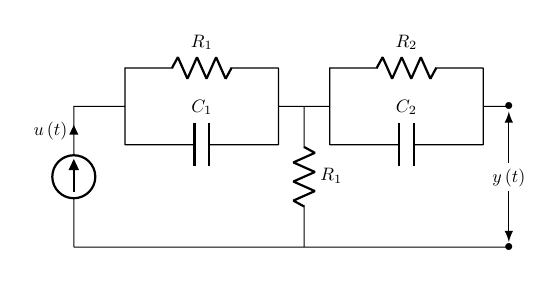
\begin{tikzpicture}[scale=0.65, transform shape]
        \path (0,0) coordinate (ref_gnd);
        \draw
            (ref_gnd) to[american current source=$u\lp t\rp$] ++(0,2.75)
                      -- (1, 2.75)
            (4,2.75) -- (5,2.75)

            (1, 2.0) -- (1, 3.5)
                to[R=\(R_1\)] ++(3,0)
            (1, 2) to[C=\(C_1\)] ++(3,0)
            (4, 2) -- (4, 3.5)

            (5, 2.0) -- (5, 3.5)
                to[R=\(R_2\)] ++(3,0)
            (5, 2) to[C=\(C_2\)] ++(3,0)
            (8, 2) -- (8, 3.5)

            (4.5, 2.75) to[R=\(R_1\)] ++(0,-2.75)
            -- (ref_gnd)

            (ref_gnd) -- (8.5, 0) node[] {$\bullet$}
            (8, 2.75) -- (8.5, 2.75) node[] {$\bullet$};

        \draw[-latex] (8.5, 1.1) node[] {} -- (8.5, 0.1) node[] {};
        \draw[-latex] (8.5, 1.65) node[below] {$y\ct{t}$} -- (8.5, 2.65) node[] {};
      \end{tikzpicture}
    \end{center}
    How are the capacitor voltages affected by input voltage $u\ct{t}$? What does $y\ct{t}$ measure?
\end{itemize}
\end{frame}


\begin{frame}[t]{Controllability}
\[ \dot{\mf{x}}\ct{t} = \mf{A}\mf{x}\ct{t} + \mf{B}\mf{u}\ct{t} \]
\[ \mf{y}\ct{t} = \mf{C}\mf{x}\ct{t} + \mf{D}\mf{u}\ct{t} \]
\vspace{-0.5cm}
\begin{itemize}
    \item Controllability tells us if a desired state can be achieved in finite time through an appropriate to choice of inputs. For this, we only have to deal with the state equation.
    
    \item \textbf{Definition}: The system or the pair $\ct{\mf{A}, \mf{B}}$ is \textbf{controllable} if for any initial state $\mf{x}_i$ and any final state $\mf{x}_f$, there exists an input $\mf{u}\ct{t}$ that transfers the initial state to the final state in finite time. Otherwise, the system is uncontrollable.

    \item It should be noted that,
    \begin{itemize}
         \item The trajectory from $\mf{x}_i$ to $\mf{x}_f$ does not matter.
         \item $\mf{u}\ct{t}$ can be anything, including impulses and derivatives of impulses.
     \end{itemize}
\end{itemize}
\end{frame}


\begin{frame}{Controllability}
\[ \dot{\mf{x}}\ct{t} = \mf{A}\mf{x}\ct{t} + \mf{B}\mf{u}\ct{t} \]
Assuming the system starts at $t=0$, the state at $t = t_f$ is given by,\vspace{-0.15cm}
\[ \mf{x}\ct{t_f} = e^{t_f\mf{A}}\mf{x}\ct{0} + \int_{0}^{t_f} e^{\ct{t_f - \tau}\mf{A}}\mf{B}\mf{u}\ct{\tau}d\tau \implies e^{-t_f\mf{A}}\mf{x}\ct{t_f} - \mf{x}\ct{0} =  \int_{0}^{t_f} e^{-\tau\mf{A}}\mf{B}\mf{u}\ct{\tau}d\tau \]

From the Cayley-Hamilton theorem we have,
\[ e^{-\tau\mf{A}} = \sum_{k=0}^{n-1}\alpha_k\ct{\tau}\mf{A}^k \implies e^{-t_f\mf{A}}\mf{x}\ct{t_f} - \mf{x}\ct{0} =  \sum_{k=0}^{n-1} \mf{A}^k\mf{B}\int_{0}^{t_f} \alpha_k\ct{\tau}\mf{u}\ct{\tau}d\tau \] \vspace{-0.15cm}
\[ \implies e^{-t_f\mf{A}}\mf{x}\ct{t_f} - \mf{x}\ct{0} =  \bmx \mf{B} & \mf{A}\mf{B} & \mf{A}^2\mf{B} & \ldots & \mf{A}^{n-1}\mf{B} \emx \bmxc \int_{0}^{t_f} \alpha_0\ct{\tau}\mf{u}\ct{\tau}d\tau \\ \vdots \\ \int_{0}^{t_f} \alpha_{n-1}\ct{\tau}\mf{u}\ct{\tau}d\tau \emx \]
\end{frame}


\begin{frame}{Controllability}
A necessary condition for achieving any arbitrary LHS is that the \textit{controllability matrix} $\mathcal{C} = \bmx \mf{B} & \mf{A}\mf{B} & \ldots & \mf{A}^{n-1}\mf{B} \emx$ is full rank. This is also a sufficient condition, which we do not show here.
\end{frame}


\begin{frame}[t]{Controllability}
\begin{itemize}
    \item A system or the pair $\ct{\mf{A}, \mf{B}}$ is controllable, if and only if the controllability matrix $\mathcal{C} = \bmx \mf{B} & \mf{A}\mf{B} & \ldots & \mf{A}^{n-1}\mf{B} \emx$ has full rank, i.e. $rank\ct{\mathcal{C}} = n$.

    \item Controllability is a system property and is not affected by the choice of coordinate system used for representing the state. Changing the basis of the state to the columns of the matrix $\mf{T}$ does not affect the rank of $\mathcal{C}$.

    \item Let $\tilde{\mf{x}} = \mf{T}^{-1}\mf{x}$, then we have $\tilde{\mf{A}} = \mf{T}^{-1}\mf{A}\mf{T}$ and $\tilde{\mf{B}} = \mf{T}^{-1}\mf{B}$. This implies that $\tilde{\mathcal{C}} = \mf{T}^{-1}\mathcal{C}$,  and $rank\ct{\tilde{\mathcal{C}}} = rank\ct{\mathcal{C}}$.
\end{itemize}
\end{frame}


\begin{frame}[t]{Controllability}
\begin{itemize}
    \item Are the following systems $\ct{\mf{A}, \mf{B}}$ controllable. (a) $\ct{\bmx 1 & 0 \\ 0 & 2 \emx, \bmx 1 \\ 1\emx}$; (b) $\ct{\bmx 1 & 0 \\ 0 & 1 \emx, \bmx 1 \\ 1\emx}$; and (c) $\ct{\bmx 1 & 0 \\ 0 & 1 \emx, \bmx 1 & -1\\ 1 & 2\emx}$.
\end{itemize}
\end{frame}
 

\begin{frame}[t]{Controllability}
When $\mf{A}$ is diagonalizable $\ct{\mf{A} = \mf{V}\mf{\Lambda}\mf{V}^{-1}}$, we have,
\[ \dot{\tilde{\mf{x}}}\ct{t} = \mf{\Lambda}\tilde{\mf{x}}\ct{t} + \tilde{\mf{B}}\mf{u}\ct{t}, \,\,\,\text{where } \tilde{\mf{x}} = \mf{V}^{-1}\mf{x} \,\, \text{ and } \tilde{\mf{B}} = \mf{V}^{-1}\mf{B}\]
\[ \tilde{\mf{x}}\ct{t_f} = e^{t_f\mf{\Lambda}}\tilde{\mf{x}}\ct{0} + \int_{0}^{t_f} e^{\ct{t_f - \tau}\mf{\Lambda}}\tilde{\mf{B}}\mf{u}\ct{\tau}d\tau \implies e^{-t_f\mf{\Lambda}}\tilde{\mf{x}}\ct{t_f} - \tilde{\mf{x}}\ct{0} =  \int_{0}^{t_f} e^{-\tau\mf{\Lambda}}\tilde{\mf{B}}\mf{u}\ct{\tau}d\tau \]

When a row of $\tilde{\mf{B}}$ is zero, then the system is not controllable, i.e. that particular first order block does not receive any input.\vspace{0.2cm}
\end{frame}


\begin{frame}[t]{Controllability}

When the two or more eigenvalue of the system are repeated, and we only have a single input to the system, then the system is not controllable (problem (b) in the previous slide).

For example, let $\mf{\Lambda} = \lambda \mf{I}$, then we have, $e^{-\lambda t_f}\tilde{\mf{x}}\ct{t_f} - \tilde{\mf{x}}\ct{0} =  \ct{\int_{0}^{t_f} e^{-\lambda\tau}u\ct{\tau}d\tau}\tilde{\mf{B}}$. Thus, the RHS can only be along the column space of $\tilde{\mf{B}}$.

\end{frame}


\begin{frame}[t]{Controllability}
When $\mf{A}$ is not diagonalizable $\ct{\mf{A} = \mf{V}\mf{J}\mf{V}^{-1}}$, where,

\[ \mf{J} = \left[
\begin{array}{cccccccc}
\lambda_1 & 1 & 0 & 0 & 0 & 0 & 0 & 0 \\
0 & \lambda_1 & 0 & 0 & 0 & 0 & 0 & 0 \\
0 & 0 & \lambda_2 & 1 & 0 & 0 & 0 & 0 \\
0 & 0 & 0 & \lambda_2 & 1 & 0 & 0 & 0 \\
0 & 0 & 0 & 0 & \lambda_2 & 0 & 0 & 0 \\
0 & 0 & 0 & 0 & 0 & \lambda_3 & \ldots & 0 \\
\vdots & \vdots & \vdots & \vdots & \vdots & \vdots & \ddots & \vdots \\
0 & 0 & 0 & 0 & 0 & 0 & \dots & \lambda_k
\end{array}
\right]
\]

\[ \dot{\tilde{\mf{x}}}\ct{t} = \mf{J}\tilde{\mf{x}}\ct{t} + \tilde{\mf{B}}\mf{u}\ct{t}, \,\,\,\text{where } \tilde{\mf{x}} = \mf{V}^{-1}\mf{x} \,\, \text{ and } \tilde{\mf{B}} = \mf{V}^{-1}\mf{B} \]

\end{frame}


\begin{frame}[t]{Controllability}


When the different Jordan blocks have distinct eigenvalues, and any of the rows of $\tilde{\mf{B}}$ corresponding the to the last row of a Jordan block is zero, then the system is not controllable, i.e. that particular Jordan order block does not receive any input.\vspace{0.2cm}

When the two or more Jordan blocks have the same eigenvalue, and we only have a single input to the system, then the system is not controllable (problem (b) in the previous slide).\vspace{0.2cm}


Is a mass $M$ in free space acted upon by a force $\mf{f} = \bmx f_1 & f_2 & f_3\emx^T$ controllable?
\end{frame}

\begin{frame}[t]{Controllability -- Discrete-time system}
\vspace{-0.2cm}
\[ \mf{x}\dt{k+1} = \mf{A}\mf{x}\dt{k} + \mf{B}\mf{u}\dt{k} \]
Assuming the system starts at $k=0$, the state at $k$ is given by,\vspace{-0.15cm}
\[ \mf{x}\dt{k} = \mf{A}^{k}\mf{x}\dt{0} + \sum_{l=0}^{k-1} \mf{A}^{k-l-1}\mf{B}\mf{u}\dt{l} \]\vspace{-0.15cm}
\[ \mf{x}\dt{k} - \mf{A}^{k}\mf{x}\dt{0} = \bmx \mf{B} & \mf{A}\mf{B} & \mf{A}^2\mf{B} & \ldots & \mf{A}^{k-1}\mf{B} \emx \bmxc \mf{u}\dt{k-1} \\ \mf{u}\dt{k-2} \\ \ldots \\ \mf{u}\dt{0} \emx = \mathcal{C}_k \tilde{\mf{u}}_{0:k-1} \]
\end{frame}

\begin{frame}[t]{Controllability -- Discrete-time system}

Assuming $\mf{x}\dt{0} = \mf{0}$, what all values can $\mf{x}\dt{k}$ take? \demoexc{2}{black}{ $\longrightarrow \mf{x}\dt{k} \in C\ct{\mathcal{C}_k}$. $\mf{x}\dt{k}$ can only be in the subspace $C\ct{\mathcal{C}_k}$.
\vspace{0.1cm}

Starting from $k=0$, the possible values $\mf{x}\dt{k}$ can take grows until, $C\ct{\mathcal{C}_{k-1}} = C\ct{\mathcal{C}_{k}}$, i.e.
\[ C\ct{\mathcal{C}_0} \subseteq C\ct{\mathcal{C}_1} \subseteq C\ct{\mathcal{C}_2 \cdots} \subseteq C\ct{\mathcal{C}_{n-1}} \subseteq C\ct{\mathcal{C}_{n}} \subseteq \mb{R}^n \]
}
\end{frame}

 
\begin{frame}[t]{Controllability -- Discrete-time system}
\begin{itemize}
    \item The subspace of reachable states can at most grow for $n$ time steps, as we add more columns from $\mf{A}^k\mf{B}$.

    \item $\mathcal{C}_{n}$ is the subspace that can be reached by the system and nothing more. Because, the columns of $\mf{A}^n\mf{B}$ are a linear combination of the columns of $\mf{B}, \mf{A}\mf{B}, \mf{A}^2\mf{B}, \ldots \mf{A}^{n-1}\mf{B}$.

    \item Thus, the system is controllable if and only if $\mathcal{C}_{n} = \mb{R}^n$, or the $rank \ct{\mathcal{C}_n} = n$.
\end{itemize}
\end{frame}


\begin{frame}{Controllability -- Discrete-time system}
\begin{itemize}
    \item In the discrete case, the controllability matrix $\mathcal{C}_n$ can also be used to determine the input sequence $\tilde{\mf{u}}_{0:n-1}$ that takes you from state $\mf{x}\dt{0}$ to $\mf{x}\dt{n}$.
    \[ \mf{x}\dt{k} - \mf{A}^{k}\mf{x}\dt{0} = \mathcal{C}_n \tilde{\mf{u}}_{0:n-1} \implies \tilde{\mf{u}}_{0:n-1} = \mathcal{C}_n^{\dagger} \ct{\mf{x}\dt{k} - \mf{A}^{k}\mf{x}\dt{0}} \]
    Where, $\mathcal{C}_n^\dagger = \mathcal{C}_n^{-1}$ for a single input system, and it is a right inverse when there are more than one inputs to the system.
\end{itemize}


Which of the following systems are controllable? (a) $\ct{\bmx 1 & 0 \\ 0 & 2 \emx, \bmx 1 \\ 1\emx}$; (b) $\ct{\bmx 1 & 0 \\ 0 & 1 \emx, \bmx 1 \\ 1\emx}$; and (c) $\ct{\bmx 1 & 0 \\ 0 & 0 \emx, \bmx 1\\ 0\emx}$.
\end{frame}


\begin{frame}{Controllability -- Discrete-time system}
When $\mf{A}$ is diagonalizable $\ct{\mf{A} = \mf{V}\mf{\Lambda}\mf{V}^{-1}}$, we have,
\[ \tilde{\mf{x}}\dt{k+1} = \mf{\Lambda}\tilde{\mf{x}}\dt{k} + \tilde{\mf{B}}\mf{u}\dt{k}, \,\,\,\text{where } \tilde{\mf{x}} = \mf{V}^{-1}\mf{x} \,\, \text{ and } \tilde{\mf{B}} = \mf{V}^{-1}\mf{B} \]
\[ \tilde{\mf{x}}\dt{k} = \mf{\Lambda}^k\tilde{\mf{x}}\dt{0} + \sum_{l=0}^{k-1} \mf{\Lambda}^{k - l - 1}\tilde{\mf{B}}\mf{u}\dt{l} \implies \tilde{\mf{x}}\dt{k} - \mf{\Lambda}^{k}\tilde{\mf{x}}\dt{0} =  \sum_{l=0}^{k-1}\mf{\Lambda}^{k-l-1}\tilde{\mf{B}}\mf{u}\ct{\tau}d\tau \]

When a row of $\tilde{\mf{B}}$ is zero, then the system is not controllable, i.e. that particular first order block does not receive any input.\vspace{0.2cm}
\end{frame}


\begin{frame}{Controllability -- Discrete-time system}
When the two or more eigenvalue of the system are repeated, and we only have a single input to the system, then the system is not controllable (problem (b) in the previous slide).

For example, let $\mf{\Lambda} = \lambda \mf{I}$, then we have, $\tilde{\mf{x}}\dt{k} - \lambda^k\tilde{\mf{x}}\dt{0} =  \ct{\sum_{l=0}^{k-1} \lambda^{k-l-1}u\dt{l}d}\tilde{\mf{B}}$. Thus, the RHS can only be along the column space of $\tilde{\mf{B}}$.
\end{frame}


\begin{frame}{Controllability -- Discrete-time system}
When $\mf{A}$ is not diagonalizable $\ct{\mf{A} = \mf{V}\mf{J}\mf{V}^{-1}}$, where,
\[ \mf{J} = \left[
\begin{array}{cccccccc}
\lambda_1 & 1 & 0 & 0 & 0 & 0 & 0 & 0 \\
0 & \lambda_1 & 0 & 0 & 0 & 0 & 0 & 0 \\
0 & 0 & \lambda_2 & 1 & 0 & 0 & 0 & 0 \\
0 & 0 & 0 & \lambda_2 & 1 & 0 & 0 & 0 \\
0 & 0 & 0 & 0 & \lambda_2 & 0 & 0 & 0 \\
0 & 0 & 0 & 0 & 0 & \lambda_3 & \ldots & 0 \\
0 & 0 & 0 & 0 & 0 & \vdots & \ddots & \vdots \\
0 & 0 & 0 & 0 & 0 & 0 & \dots & \lambda_k
\end{array}
\right]
\]

\[ \tilde{\mf{x}}\dt{k+1} = \mf{J}\tilde{\mf{x}}\dt{k} + \tilde{\mf{B}}\mf{u}\dt{k}, \,\,\,\text{where } \tilde{\mf{x}} = \mf{V}^{-1}\mf{x} \,\, \text{ and } \tilde{\mf{B}} = \mf{V}^{-1}\mf{B} \]
\end{frame}


\begin{frame}[t]{Controllability -- Discrete-time system}
When the different Jordan blocks have distinct eigenvalues, and any of the rows of $\tilde{\mf{B}}$ corresponding the to the last row of a Jordan block is zero, then the system is not controllable, i.e. that particular Jordan order block does not receive any input.
\vspace{0.5cm}

When the two or more Jordan blocks have the same eigenvalue, and we only have a single input to the system, then the system is not controllable (problem (b) in the previous slide).
\end{frame}


\begin{frame}[t]{Observability}
\[ \dot{\mf{x}}\ct{t} = \mf{A}\mf{x}\ct{t} + \mf{B}\mf{u}\ct{t} \]
\[ \mf{y}\ct{t} = \mf{C}\mf{x}\ct{t} + \mf{D}\mf{u}\ct{t} \]
\vspace{-0.5cm}
\begin{itemize}
    \item Observability tells us if we can determine all the states of a system using our knowledge of the inputs and the outputs to the system over a finite duration of time. For this, we only have to deal with the measurement equation.
    
    \item \textbf{Definition}: The system or the pair $\ct{\mf{A}, \mf{C}}$ is \textbf{observable} if every state $\mf{x}\ct{0}$ can be determined from the observation of the output $\mf{y}\ct{t}$ over a finite period of time, $0 \leq t \leq t_1$. Otherwise, the system is unobservable.

    \item Observability is important to be able to estimate states that cannot be directly measured. Knowledge of the states is essential for implementing state feedback controllers.
\end{itemize}
\end{frame}


\begin{frame}[t]{Observability}
\[ \mf{y}\ct{t} = \mf{C}\mf{x}\ct{t} + \mf{D}\mf{u}\ct{t} \]
Assuming the system starts at $t=0$, the output at time $t$ is given by,\vspace{-0.15cm}
\[ \mf{y}\ct{t} = \mf{C}e^{t\mf{A}}\mf{x}\ct{0} + \int_{0}^{t} \mf{C}e^{\ct{t - \tau}\mf{A}}\mf{B}\mf{u}\ct{\tau}d\tau + \mf{D}\mf{u}\ct{t} \]

Let $\hat{\mf{y}}\ct{t} = \mf{y}\ct{t} - \int_{0}^{t} \mf{C}e^{\ct{t - \tau}\mf{A}}\mf{B}\mf{u}\ct{\tau}d\tau - \mf{D}\mf{u}\ct{t}$. Then we have,\vspace{-0.25cm}
\[ \hat{\mf{y}}\ct{t} = \mf{C}e^{t\mf{A}}\mf{x}\ct{0} \implies \hat{\mf{y}}\ct{t} = \sum_{k=0}^{n-1} \alpha_k\ct{t}\mf{C}\mf{A}^k\mf{x}\ct{0} =  \bmxc \alpha_0\ct{t}\mf{I}_{r} & \ldots & \alpha_{n-1}\ct{t}\mf{I}_{r} \emx \bmxc \mf{C} \\ \mf{C}\mf{A} \\ \mf{C}\mf{A}^2 \\ \vdots \\ \mf{C}\mf{A}^{n-1} \emx \mf{x}\ct{0}  \]
\end{frame}


\begin{frame}{Observability}
A necessary condition to uniquely determine $\mf{x}\ct{0}$ from $\tilde{\mf{y}}\ct{t}$ is that the \textit{observability matrix} $\mathcal{O} = \bmx \mf{C} & \mf{C}\mf{A} & \ldots & \mf{C}\mf{A}^{n-1} \emx^T$ is full rank. This is also a sufficient condition, which we do not show here.
\end{frame}


\begin{frame}[t]{Observability}
\begin{itemize}
    \item A system or the pair $\ct{\mf{A}, \mf{C}}$ is controllable, if and only if the controllability matrix $\mathcal{O} = \bmx \mf{C} & \mf{C}\mf{A} & \ldots & \mf{C}\mf{A}^{n-1} \emx^T$ has full rank, i.e. $rank\ct{\mathcal{O}} = n$.

    \item Observability is a system property and is not affected by the choice of coordinate system used for representing the state. Changing the basis of the state to the columns of the matrix $\mf{T}$ does not affect the rank of $\mathcal{O}$.

    \item Let $\tilde{\mf{x}} = \mf{T}^{-1}\mf{x}$, then we have $\tilde{\mf{A}} = \mf{T}^{-1}\mf{A}\mf{T}$ and $\tilde{\mf{C}} = \mf{B}\mf{T}$. This implies that $\tilde{\mathcal{O}} = \mathcal{O}\mf{T}$, and $rank\ct{\tilde{\mathcal{O}}} = rank\ct{\mathcal{O}}$.
\end{itemize}
\end{frame}


\begin{frame}[t]{Observability}
\begin{itemize}
    \item When $\mf{A}$ is diagonalizable $\ct{\mf{A} = \mf{V}\mf{\Lambda}\mf{V}^{-1}}$, we have, $\hat{\mf{y}}\ct{t} = \tilde{\mf{C}}e^{t\mf{\Lambda}}\tilde{\mf{x}}\ct{0}$

    \begin{itemize}
        \item When a column of $\tilde{\mf{C}}$ is zero, then the system is not observable, i.e. that particular first order block does not contribute anything to the output.\vspace{0.2cm}

        \item When the two or more eigenvalue of the system are repeated, and the system has only one output, then the system is not observable.
    \end{itemize}
\end{itemize}
\end{frame}


\begin{frame}{Observability -- Discrete-time system}
\vspace{-0.2cm}
\[ \mf{y}\dt{k} = \mf{C}\mf{x}\dt{k} + \mf{D}\mf{u}\dt{k} \]
Assuming the system starts at $k=0$, the output at $k$ is given by,\vspace{-0.15cm}
\[ \mf{y}\dt{k} = \mf{C}\mf{A}^{k}\mf{x}\dt{0} + \sum_{l=0}^{k-1} \mf{C}\mf{A}^{k-l-1}\mf{B}\mf{u}\dt{l} + \mf{D}\mf{u}\dt{k} \]\vspace{-0.15cm}

Let $\hat{\mf{y}}\dt{k} = \mf{y}\dt{k} - \sum_{l=0}^{k-1} \mf{C}\mf{A}^{k-l-1}\mf{B}\mf{u}\dt{l} - \mf{D}\mf{u}\dt{k}$. Then we have,\vspace{-0.15cm}
\[ \hat{\mf{y}}\dt{k} = \mf{C}\mf{A}^k\mf{x}\dt{0} \implies \bmxc \hat{\mf{y}}\dt{0}\\ \hat{\mf{y}}\dt{1}\\ \vdots \\\hat{\mf{y}}\dt{k} \emx = \bmxc \mf{C} \\ \mf{C}\mf{A} \\ \vdots \\ \mf{C}\mf{A}^{k} \emx \mf{x}\ct{0} = \mathcal{O}_k\mf{x}\dt{0}\]

When $rank\ct{\mathcal{O}_k} = n$, then we can uniquely determine any $\mf{x}\ct{0}$ from $\mf{y}\dt{k}$. 

Starting with $k=0$, the $rank\ct{\mathcal{O}_k}$ can grow till $k = n-1$.
\end{frame}

 
\begin{frame}{Observability -- Discrete-time system}
\begin{itemize}
    \item In the discrete case, the observability matrix $\mathcal{O}_{n-1}$ can also be used to determine the the state $\mf{x}\ct{0}$.
    \[ \hat{\mf{y}}\dt{n-1} = \mathcal{O}_{n-1}\mf{x}\dt{0} \implies \mf{x}\dt{0} = \mathcal{O}_{n-1}^\dagger\hat{\mf{y}}\dt{n-1} \]
    Where, $\mathcal{O}_{n-1}^\dagger = \mathcal{O}_{n-1}^{-1}$ for a single output system, and it is a left inverse when there is more than one output from the system.

    \item When $\mf{A}$ is diagonalizable $\ct{\mf{A} = \mf{V}\mf{\Lambda}\mf{V}^{-1}}$, we have, $\hat{\mf{y}}\dt{k} = \tilde{\mf{C}}\mf{\Lambda}^k\tilde{\mf{x}}\dt{0}$

    \begin{itemize}
        \item When a column of $\tilde{\mf{C}}$ is zero, then the system is not observable, i.e. that particular first order block does not contribute anything to the output.\vspace{0.2cm}

        \item When the two or more eigenvalue of the system are repeated, and the system has only one output, then the system is not observable.
    \end{itemize}
\end{itemize}
\end{frame}
\end{document}
\end{document}